\xchapter{OUR PROOF OF CONCEPT SOLUTION FOR PUBLIC COMMUNICATION OF EMERGENCIES}{}\label{sec:rescuerNews}

\section{RESCUER Project}

Our research fits in the scope of a larger research project named RESCUER \footnote{\url{http://www.rescuer-project.org/}}, which aims at developing an inter-operable solution that supports command centres in quickly managing emergencies and crisis based on reliable and intelligent analysis of crowdsourcing information mashed up with open data \citep{villela2014smart}\citep{villela2018}. Two application scenarios are under investigation and support emergency and crisis management in: i) Industrial areas, such as chemical parks; and ii) Large-scale events, such as the Olympic Games.

\begin{figure}[ht!]
\begin{center}
  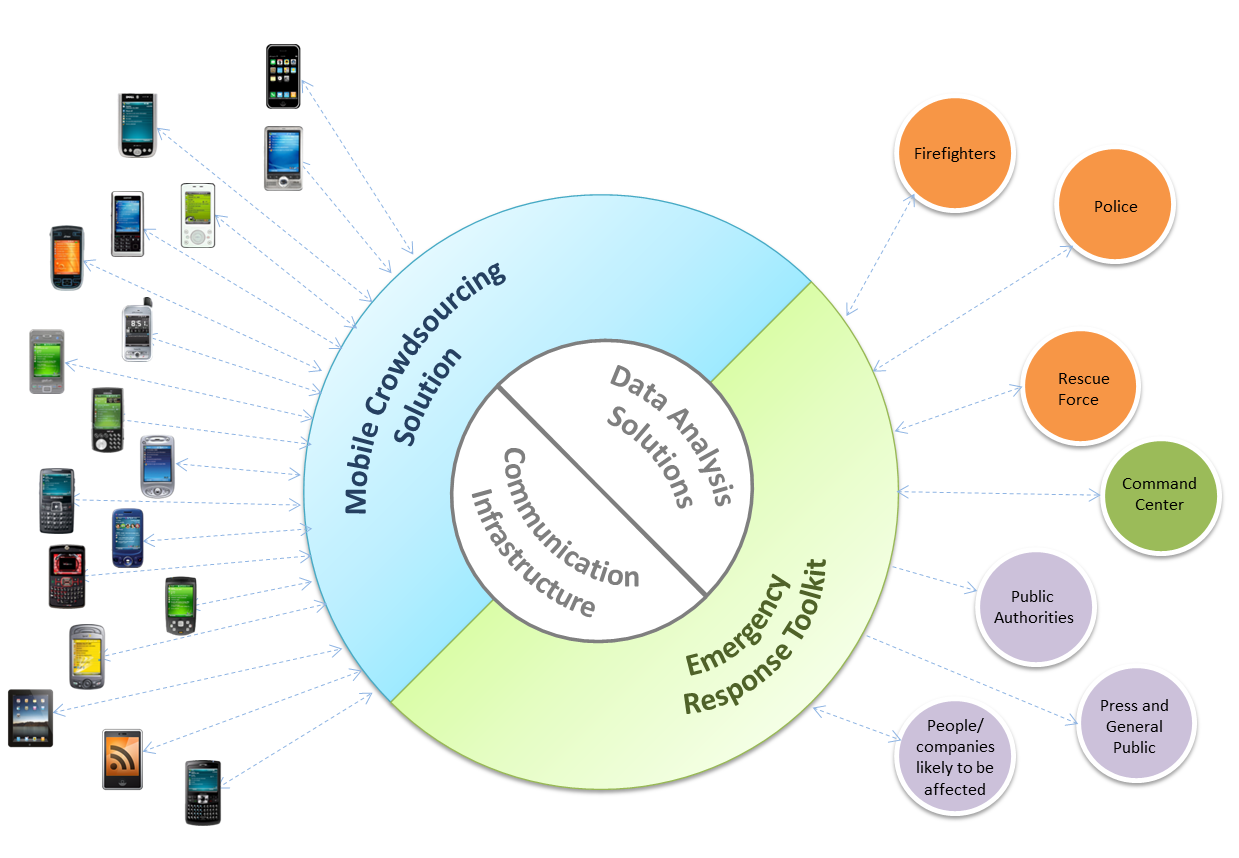
\includegraphics[width=0.75\linewidth, keepaspectratio]{images/rescuerConcept.PNG}
\caption{RESCUER Conceptual Model \citep{villela2014smart}}
\label{fig:rescuerConcept}
\end{center}
\end{figure}

Figure \ref{fig:rescuerConcept} presents the conceptual view of the Rescuer project. The project was divided into four main components: Mobile Crowdsourcing Solution (MCS), Data Analysis Solutions (DAS); Communication Infrastructure and Emergency Response Toolkit (ERTK). 

The MCS \citep{nass2018interaction} is way to receive or send information by the crowd. The users of MCS can be an operational force actuating in mitigating the effects of the crisis or a civilian near the incident place.

In order to guarantee that the information will be sent or received in a suitable time and even when traditional communication infrastructure are overloaded, the Rescuer Project has the Communication Infrastructure module. Inside of this module, we have the Rescuer Emergency State Builder (RESCUER ESB) \citep{pereiraetall2017}, a component designed to aggregate contextual information about emergencies from multiple data sources.

The DAS module is responsible to integrate data from different profiles as well as for combining, filtering, and data analysing \citep{chino2015bowfire} crowdsourcing information mashed up with open data. 

Finally, the ERTK module provide the command centre with updated and relevant information, in the appropriate format, to support decision-making in the different phases of an emergency and allow the dissemination of orientations to the affected people and reliable information in the course of emergency.

\Section{RESCUER News - A variability based solution for public communication of emergencies}

\begin{figure}
\centering
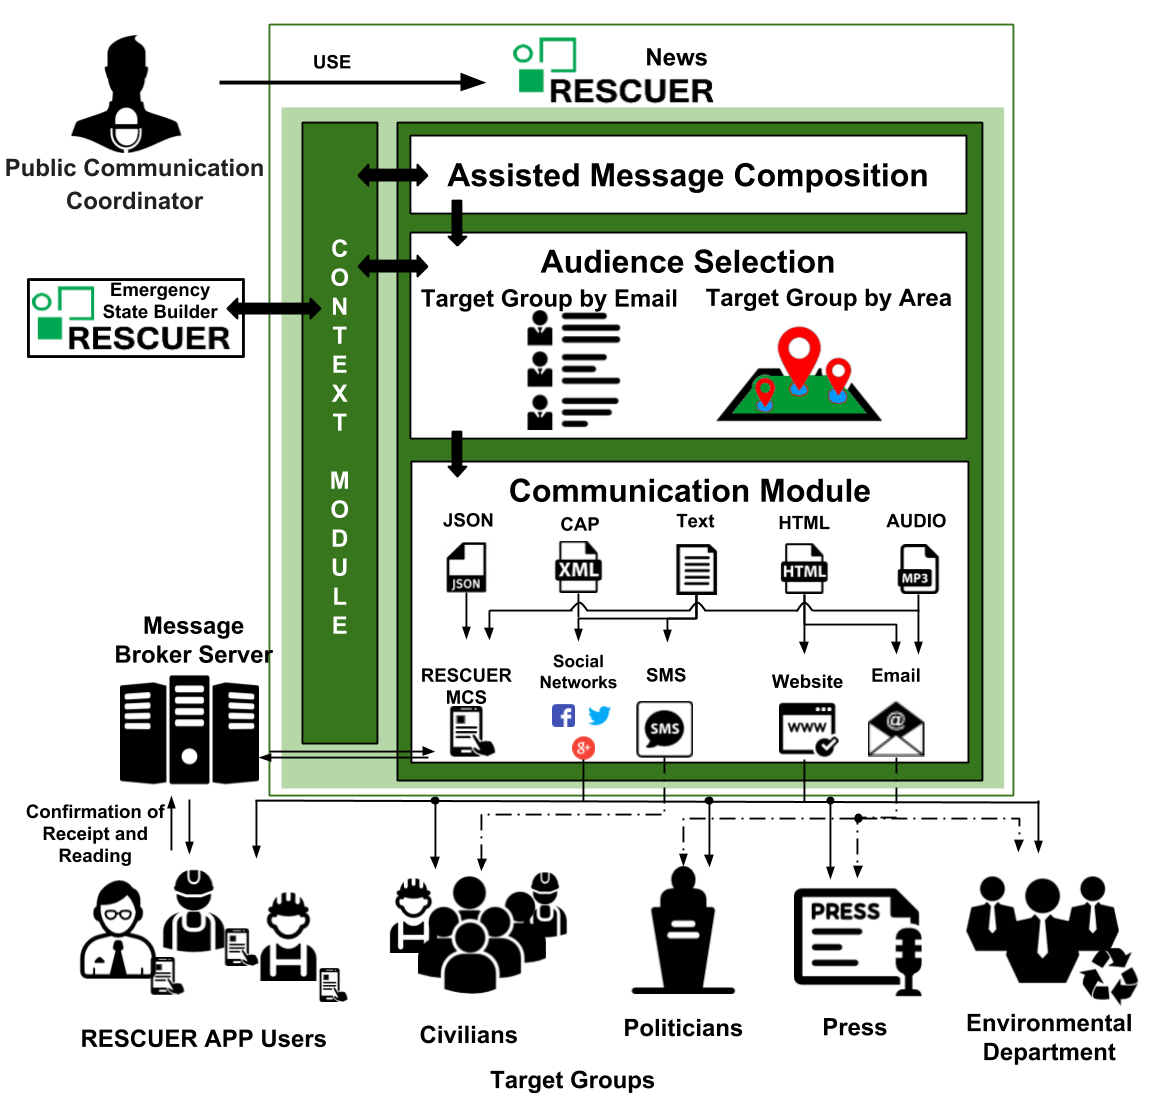
\includegraphics[width=0.75\linewidth]{images/RescuerNewsConcept}
\caption{RESCUER News Overview}
\label{fig:rescuerOverview}
\end{figure} 

The RESCUER News was develop inside of the RESCUER Project, more specifically, as the public communication solution of the ERTK module. RESCUER News represents an real example of an implementation of our variability model for Public Communication of Emergencies.   

The RESCUER News was built to help the public communication team in the task of generating and disseminating public communications during an emergency. To do this, we design our solution to contemplate all process of public communication in just 4 steps.

Figure \ref{fig:rescuerOverview} shows an overview of RESCUER News. The communicator will use the system. The system will start by requesting the current emergency state to RESCUER ESB, because this information is used to find the best template and also to provide variable information to complete the public communication. The user then selects options offered by the template as desired and makes the final adjustments by freely editing the text. At this point, the system generates messages in specific formats for each of the chosen communication channels, allows the inclusion of new stakeholders in the target audience and delivers the public communication to the chosen target audience.

\begin{figure*}[!h]
\centering
\subfloat[User interface to setting the basic information about the emergency]{
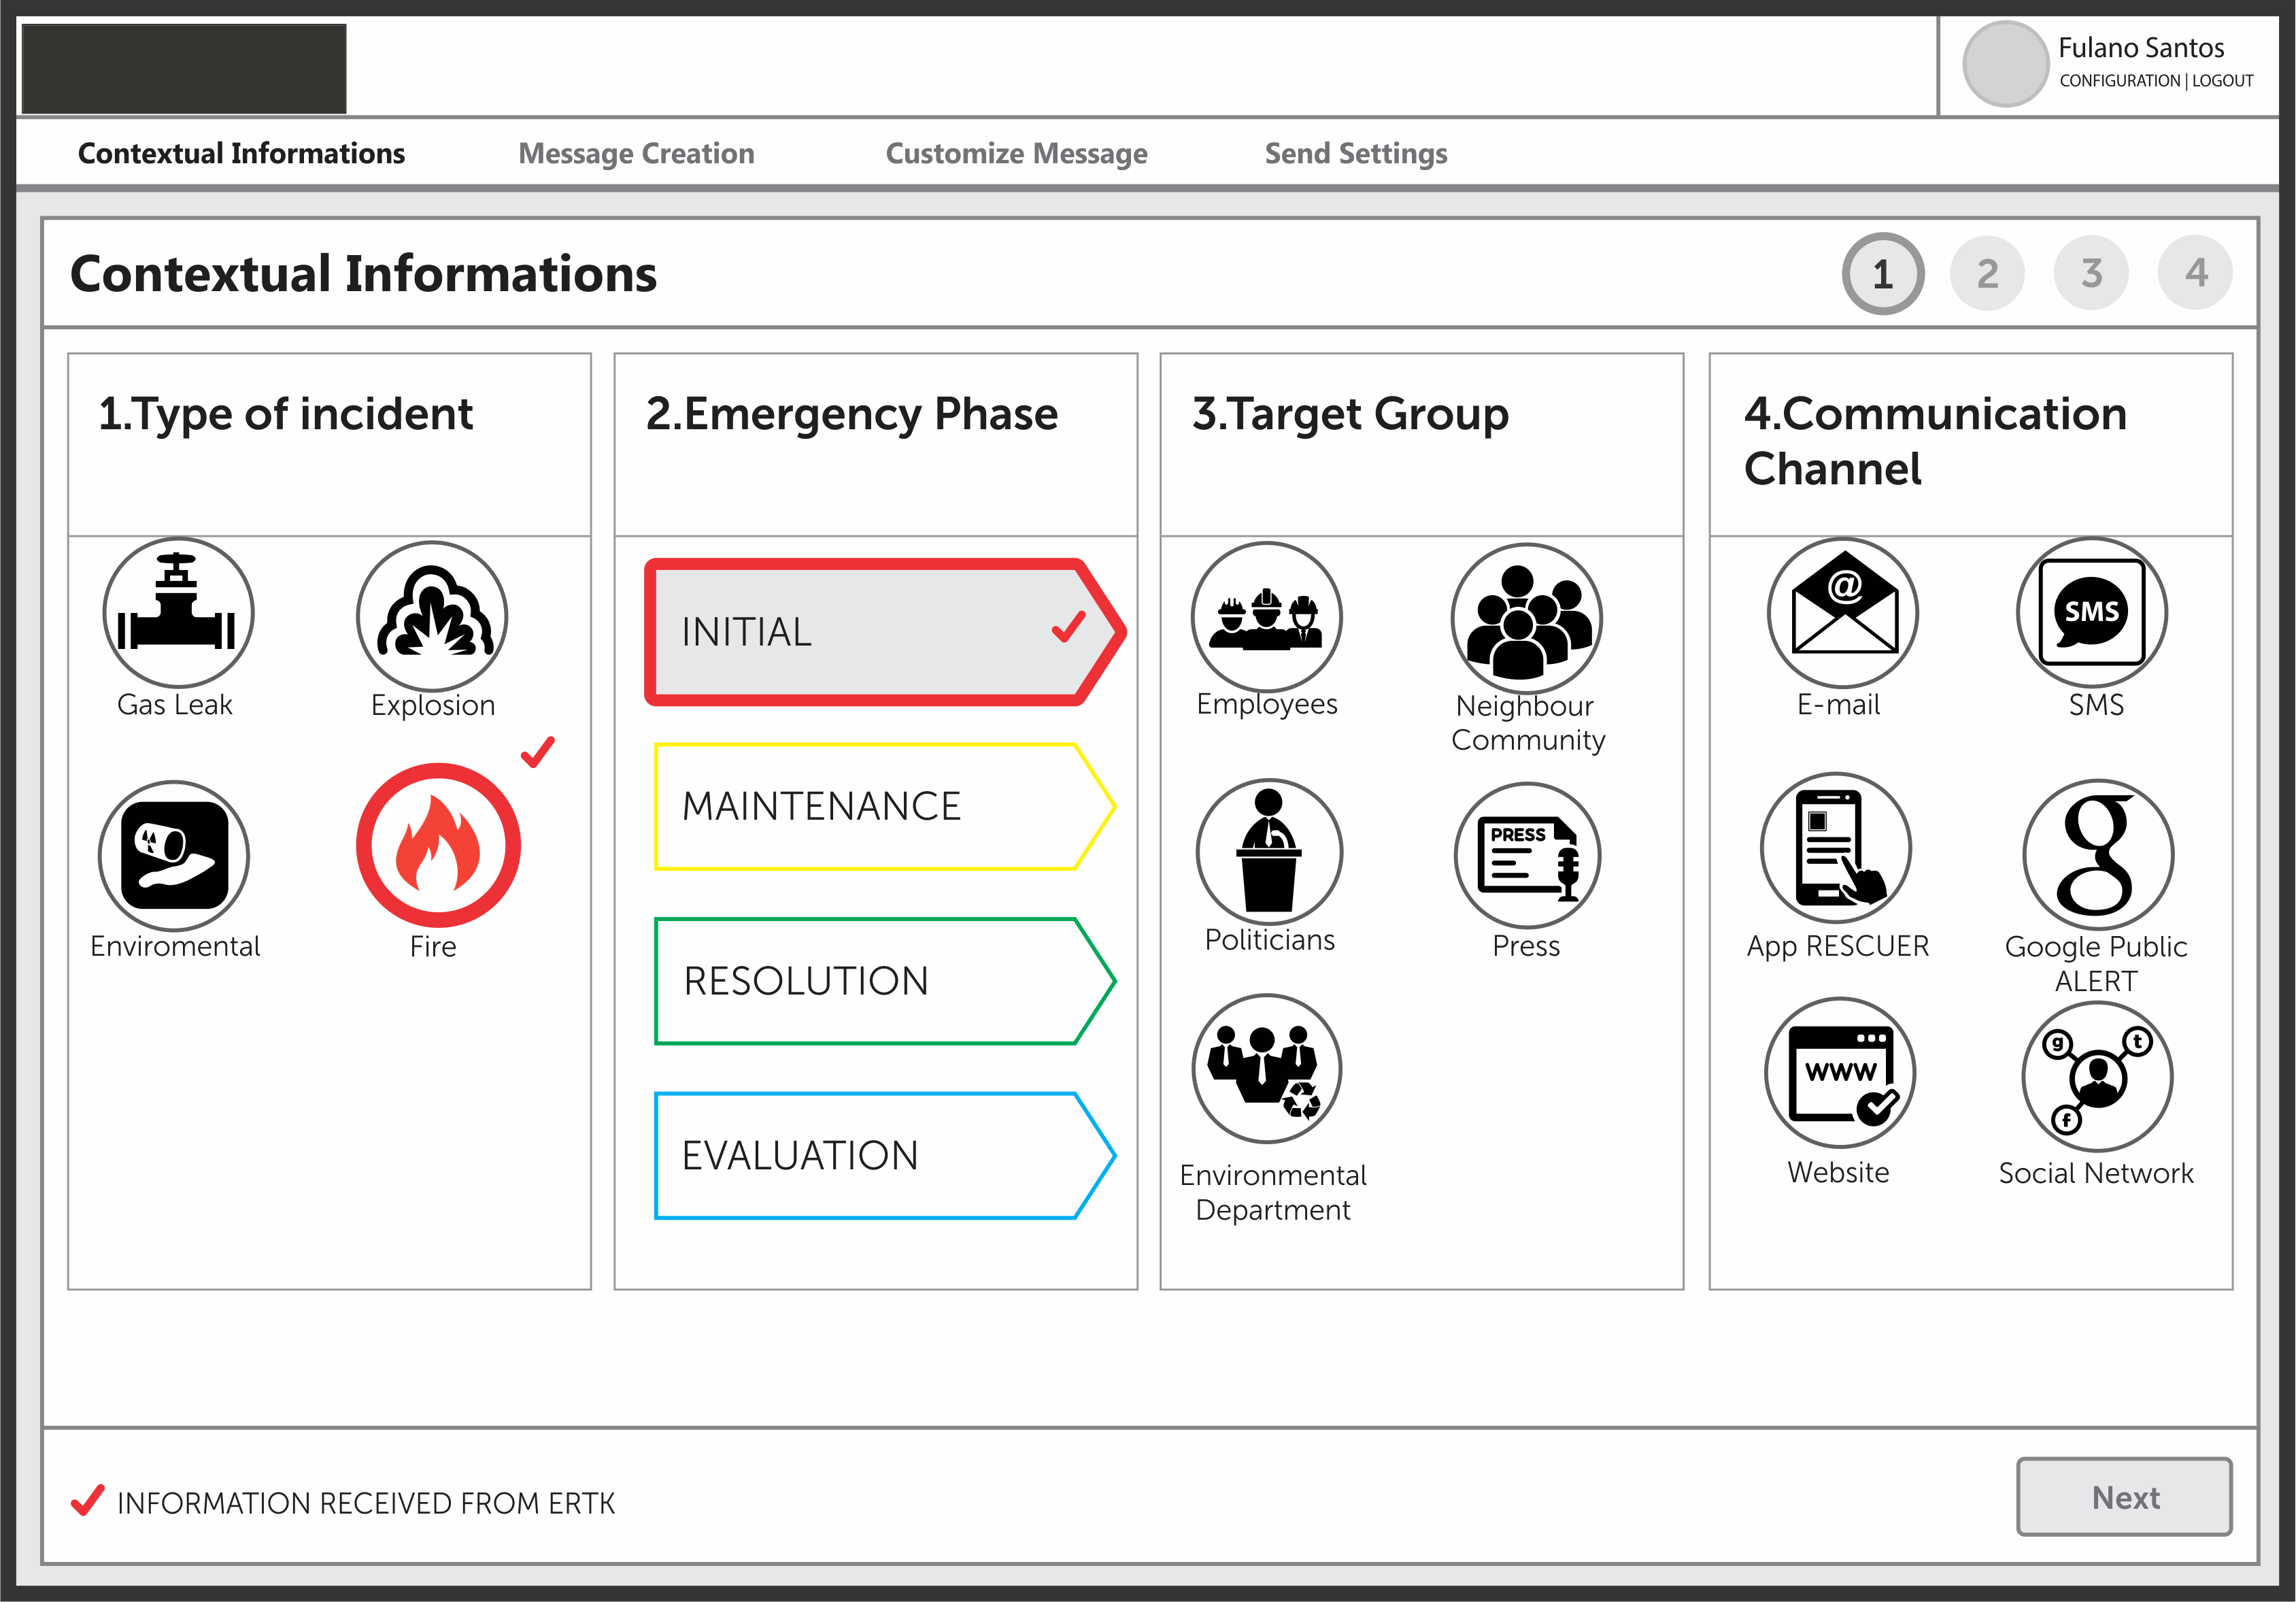
\includegraphics[width=0.45\linewidth]{images/step1.png}
\label{fig:step1}
}
\quad %espaco separador
\subfloat[Assisted Message Edition screen configured to build a public communication informing the occurrence episode of riot inside of the stadium]{
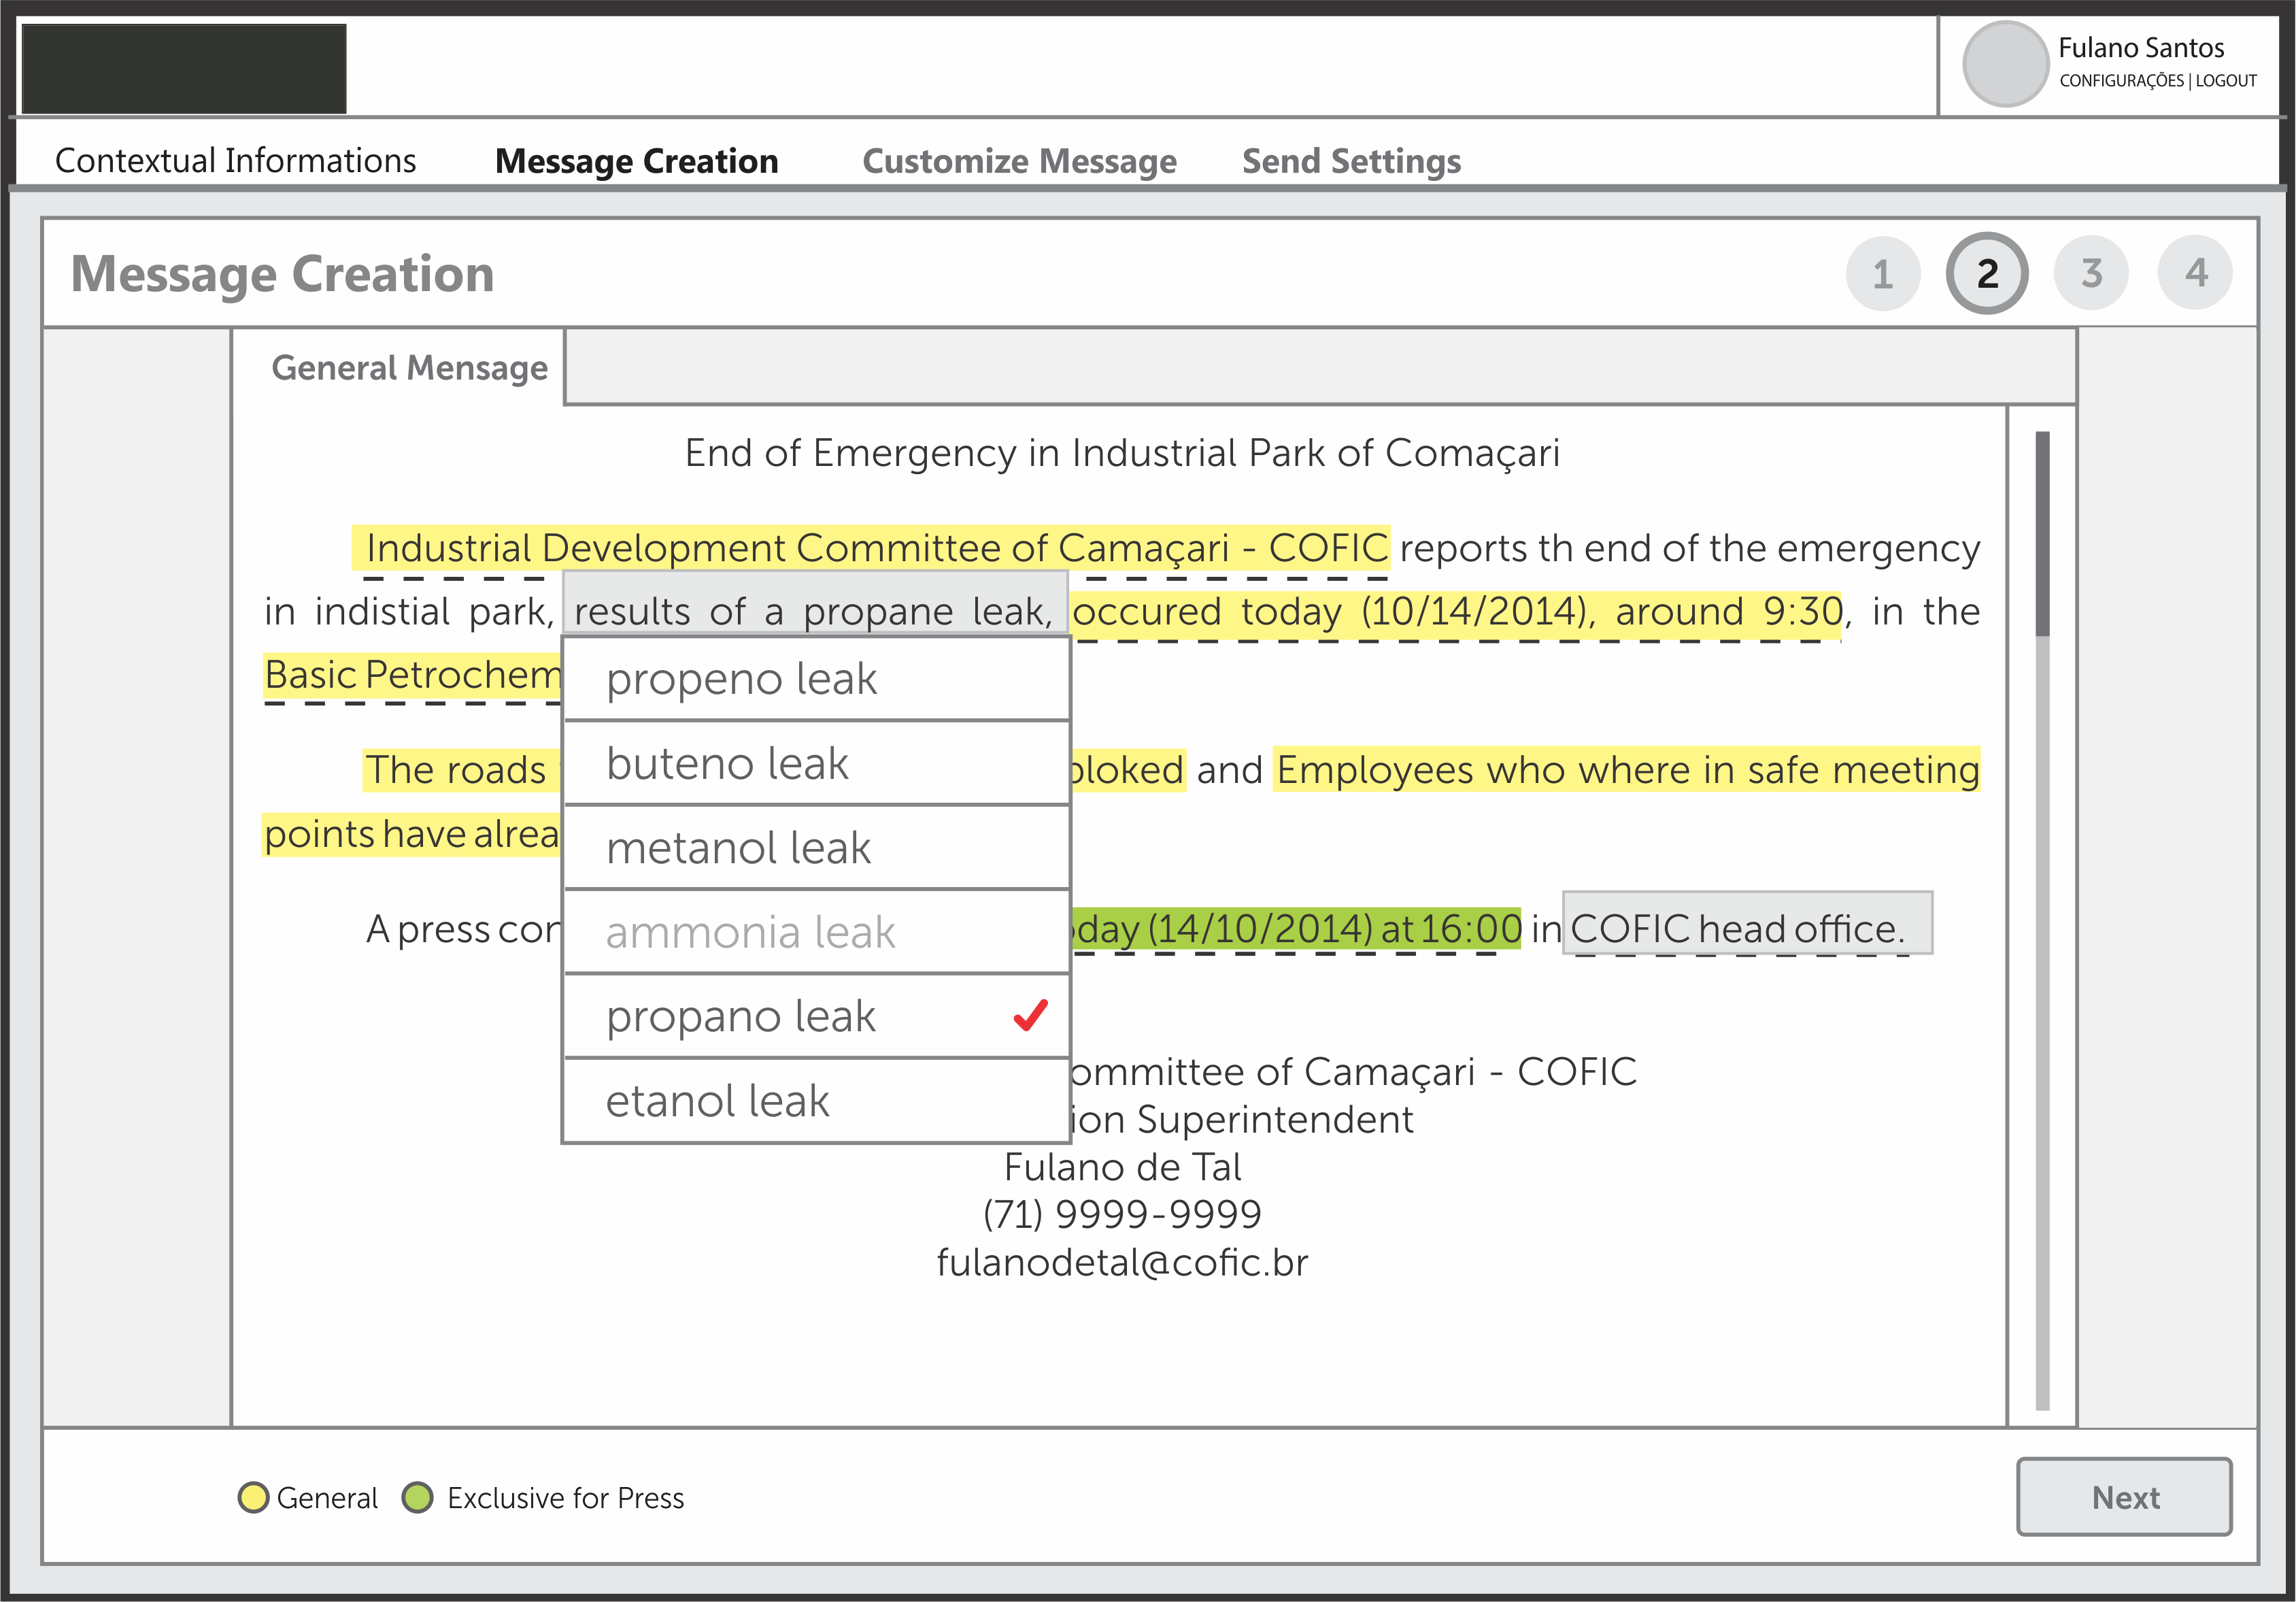
\includegraphics[width=0.45\linewidth]{images/step2.png}
\label{fig:step2}
}
\quad %espaco separador
\subfloat[User interface to assisted message edition of public communications]{
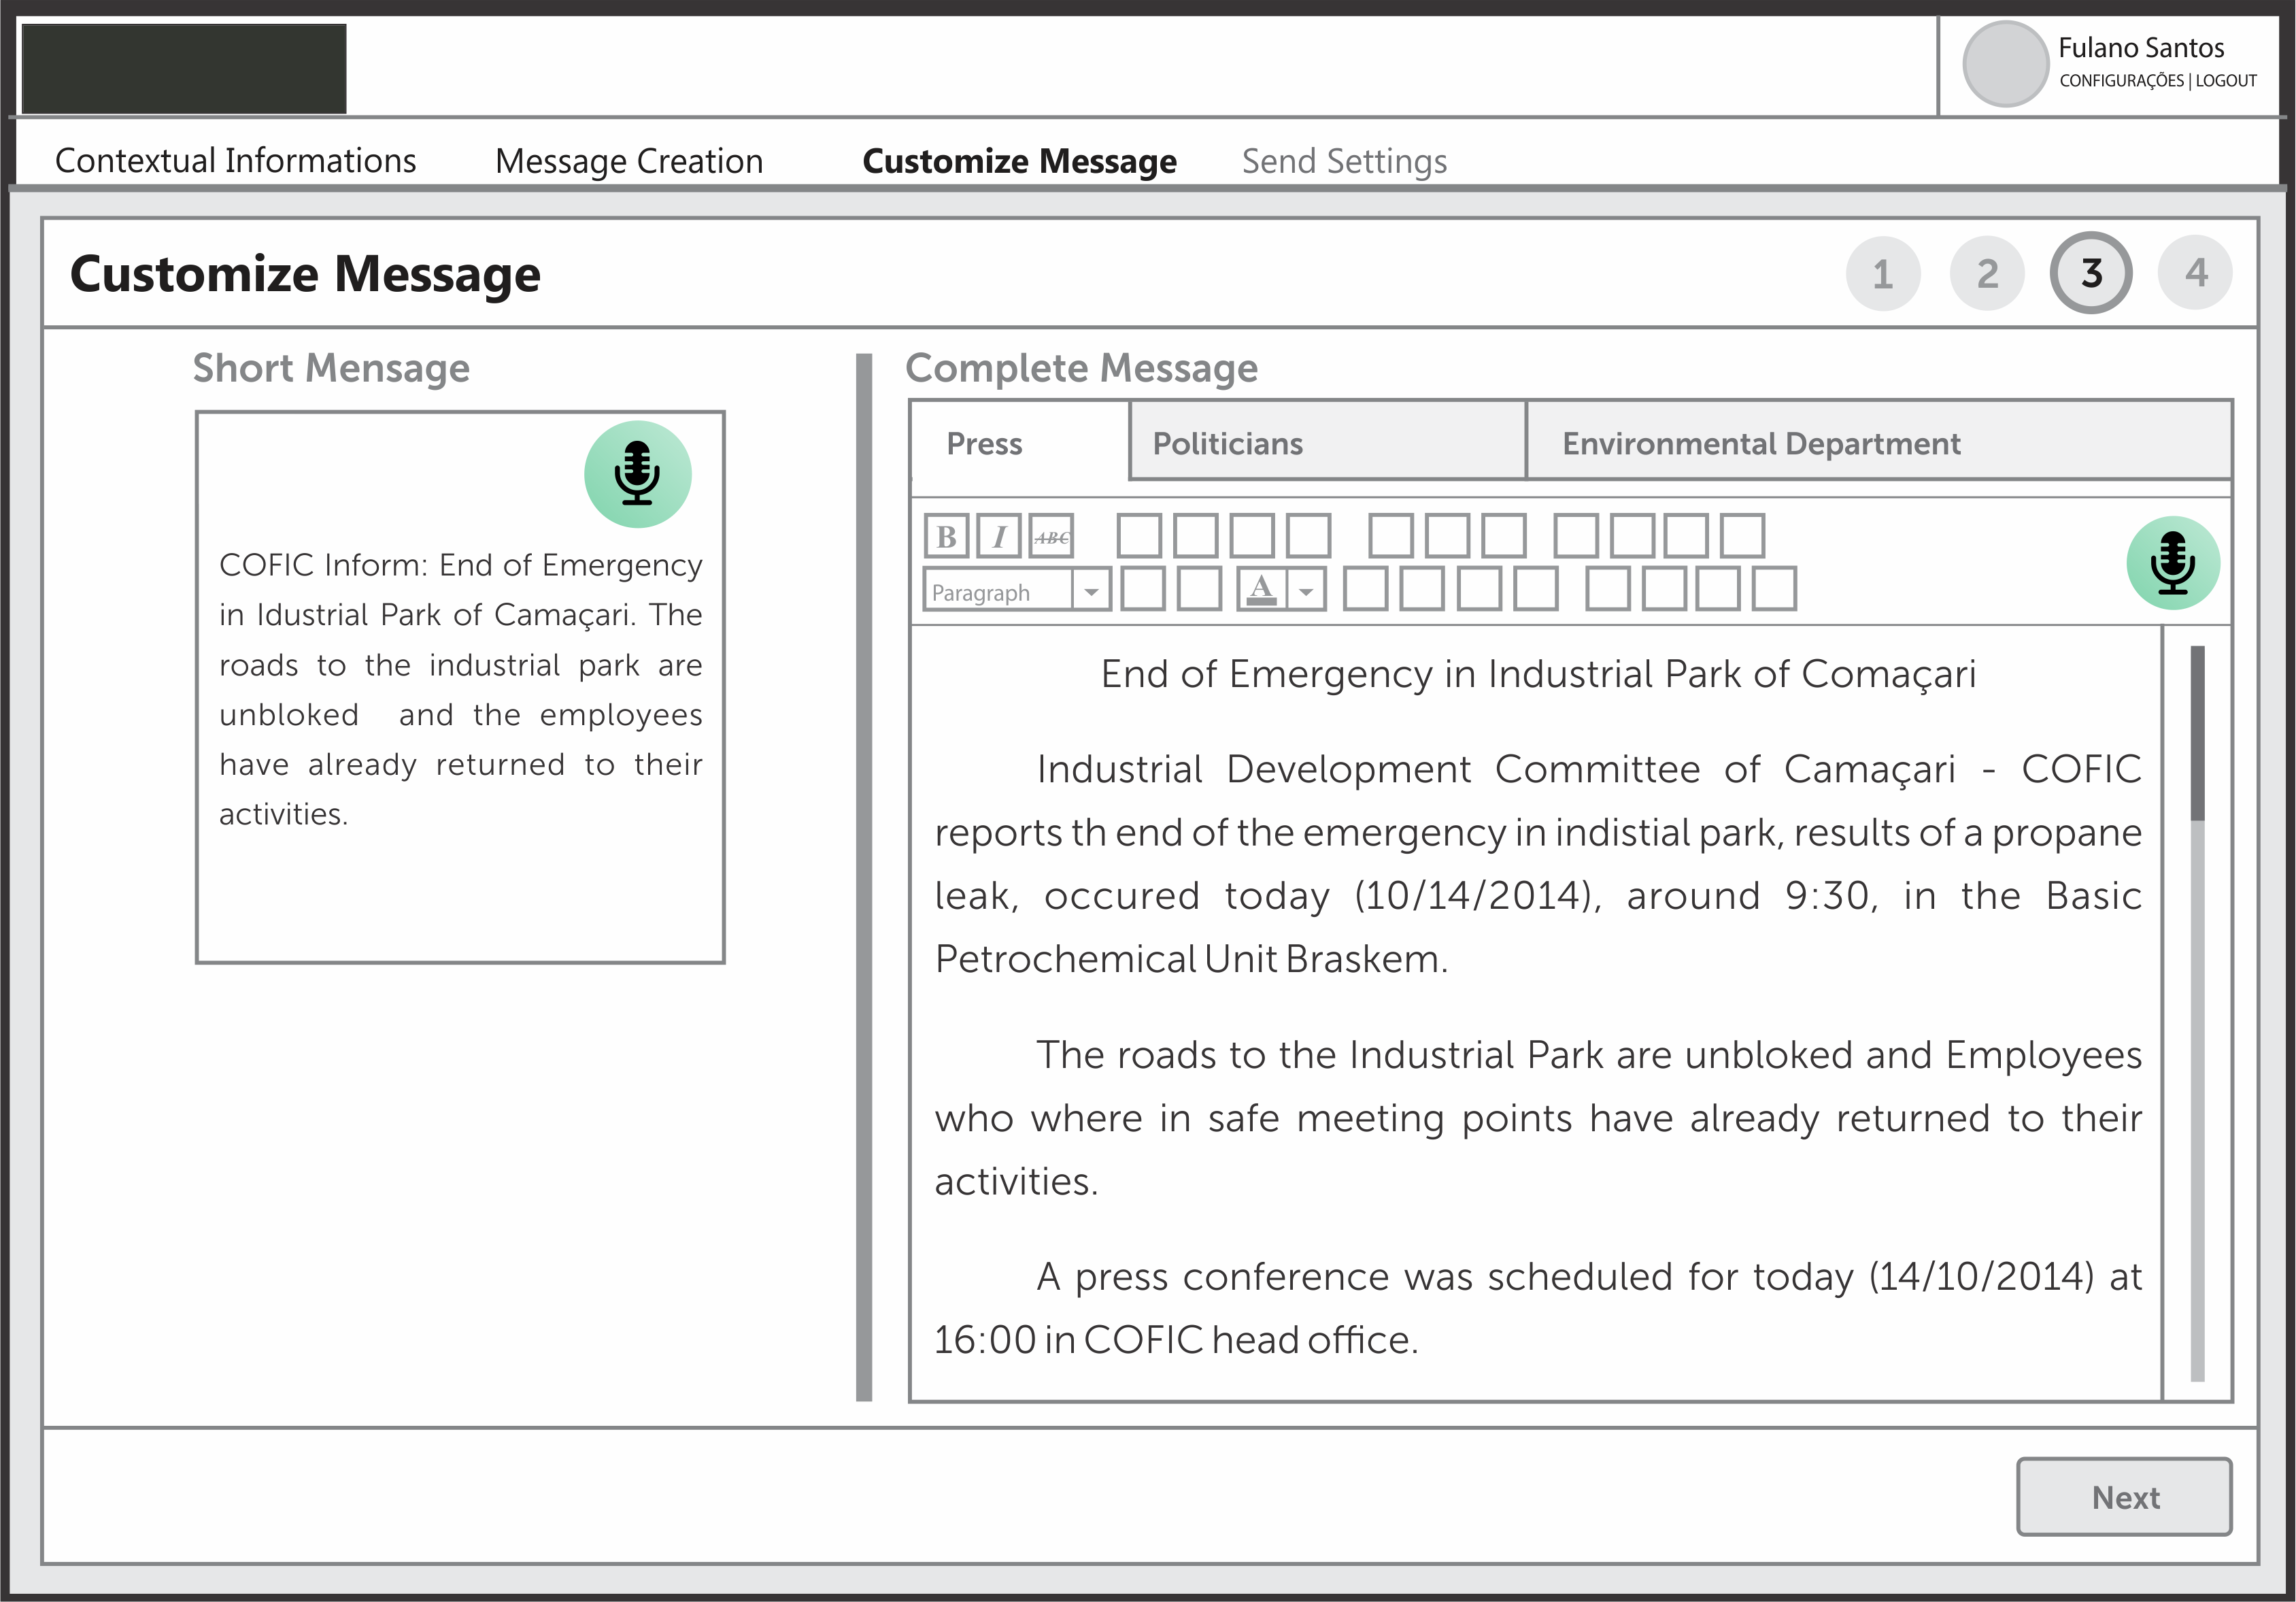
\includegraphics[width=0.45\linewidth]{images/step3.png}
\label{fig:step3}
}
\quad %espaco separador
\subfloat[User interface of target audience sending settings]{
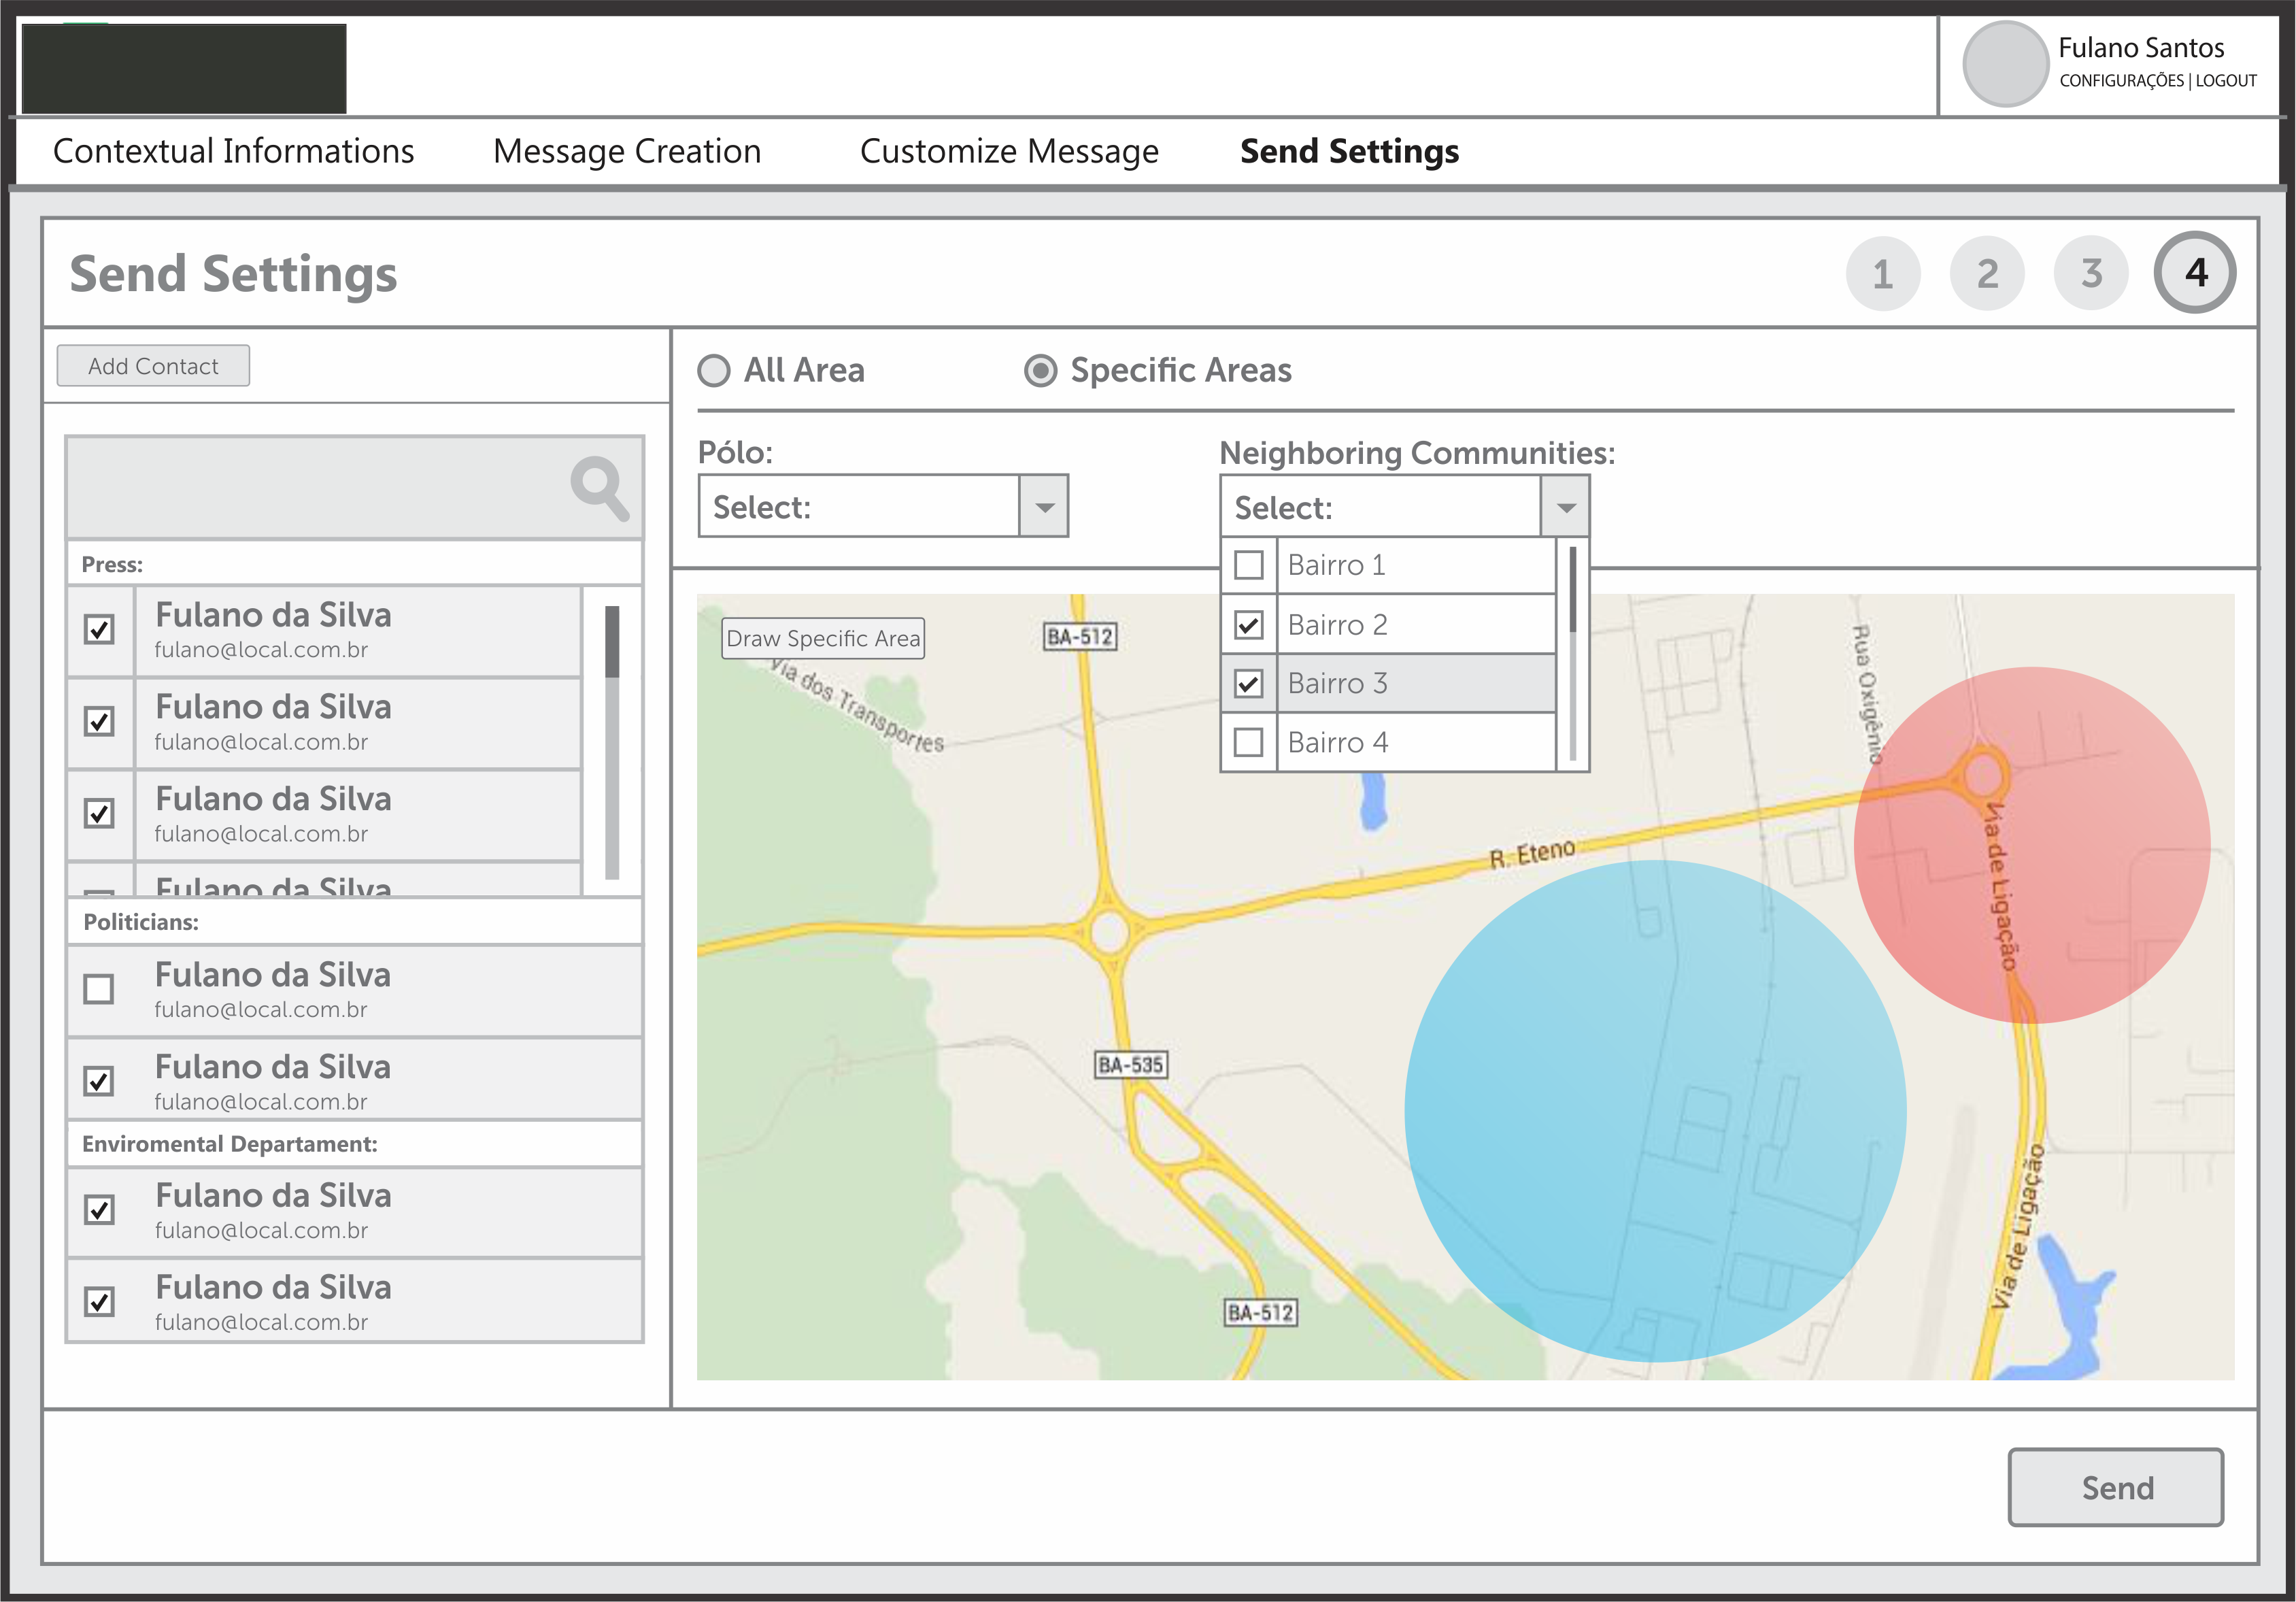
\includegraphics[width=0.45\linewidth]{images/step4.png}
\label{fig:step4}
}
\caption{RESCUER News mookups}
\label{fig:rescuerNews}
\end{figure*}

% \begin{figure}[h]
% \centering
% 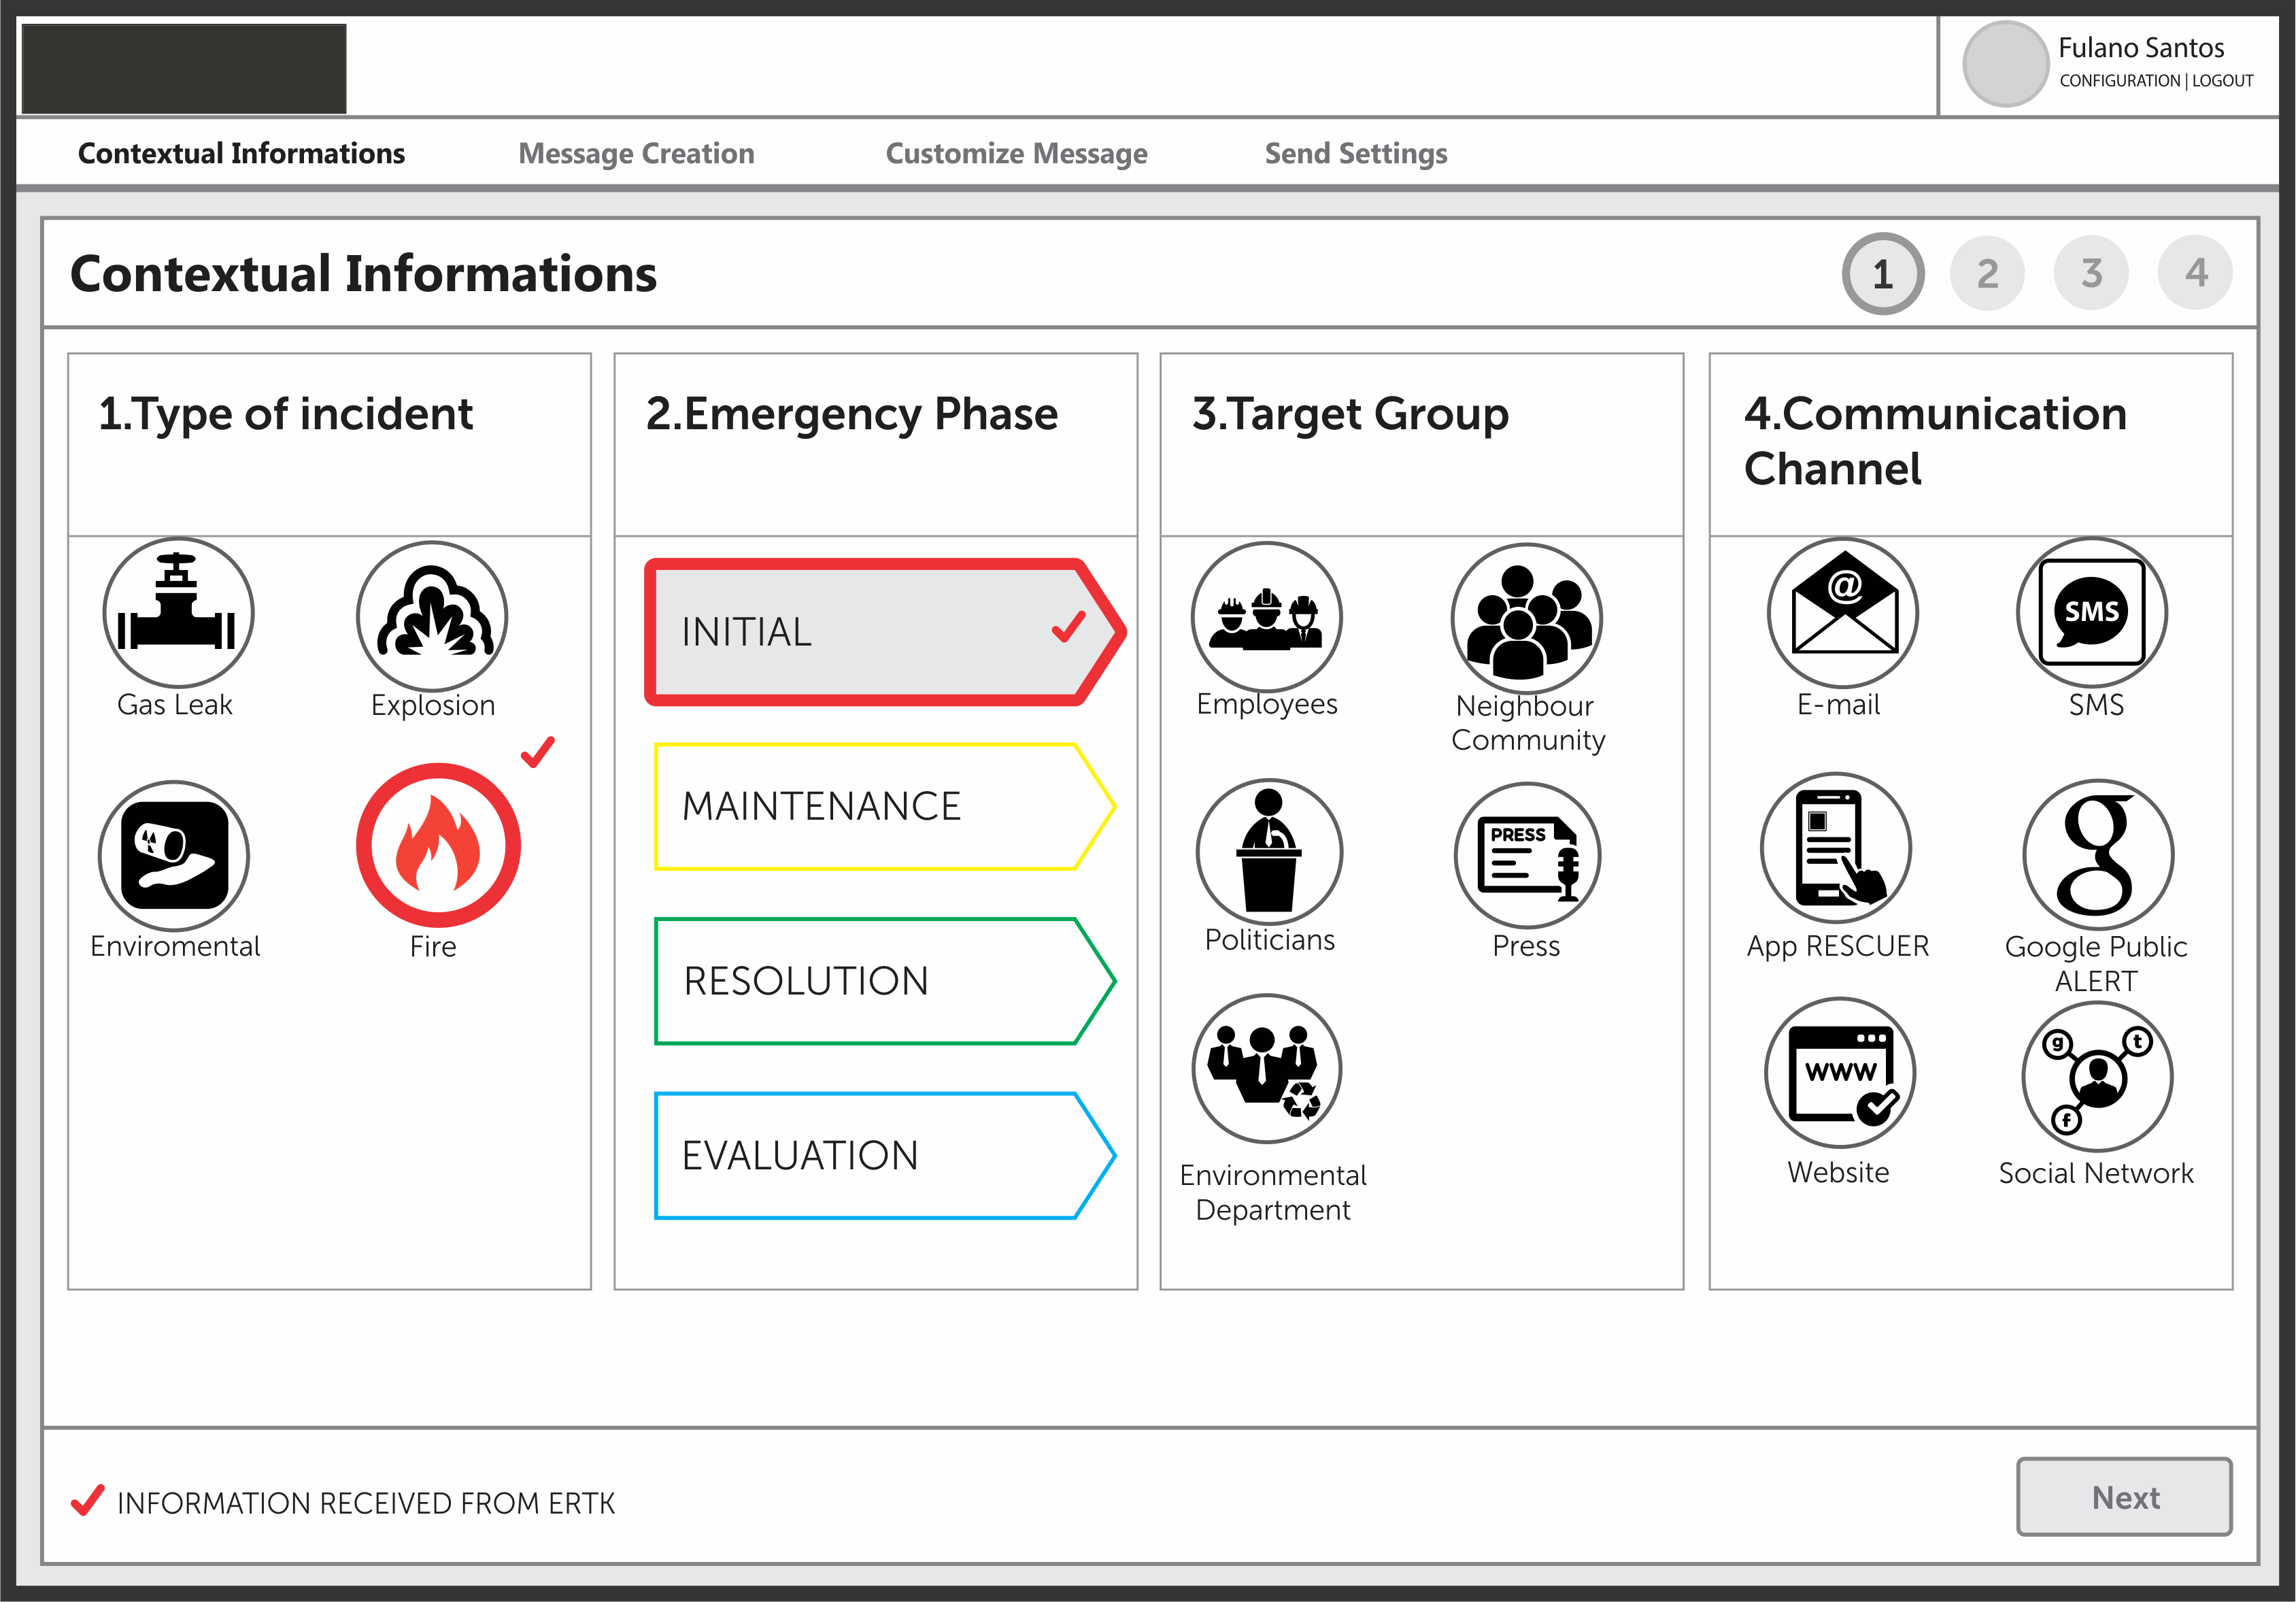
\includegraphics[width=\linewidth]{images/step1.png}
% \caption{User interface to setting the basic information about the emergency}
% \label{fig:step1}
% \end{figure}

In this first step, RESCUER News requests information about the current emergency state, such as emergency type, the current phase of emergency (emergency status), occurrence time, the name of affected company (incident location), and number of injuries or fatalities. If the emergency state is obtained from the ERTK, the system will use the emergency type and the current phase of the emergency to search the best communication template in the following step.
Then the user chooses the targets groups and the communication channels to be used. Figure \ref{fig:step1} presents the user interface for this step. The information coming from Rescuer ESB is marked with the red check marks.


% \begin{figure}
% \centering
% 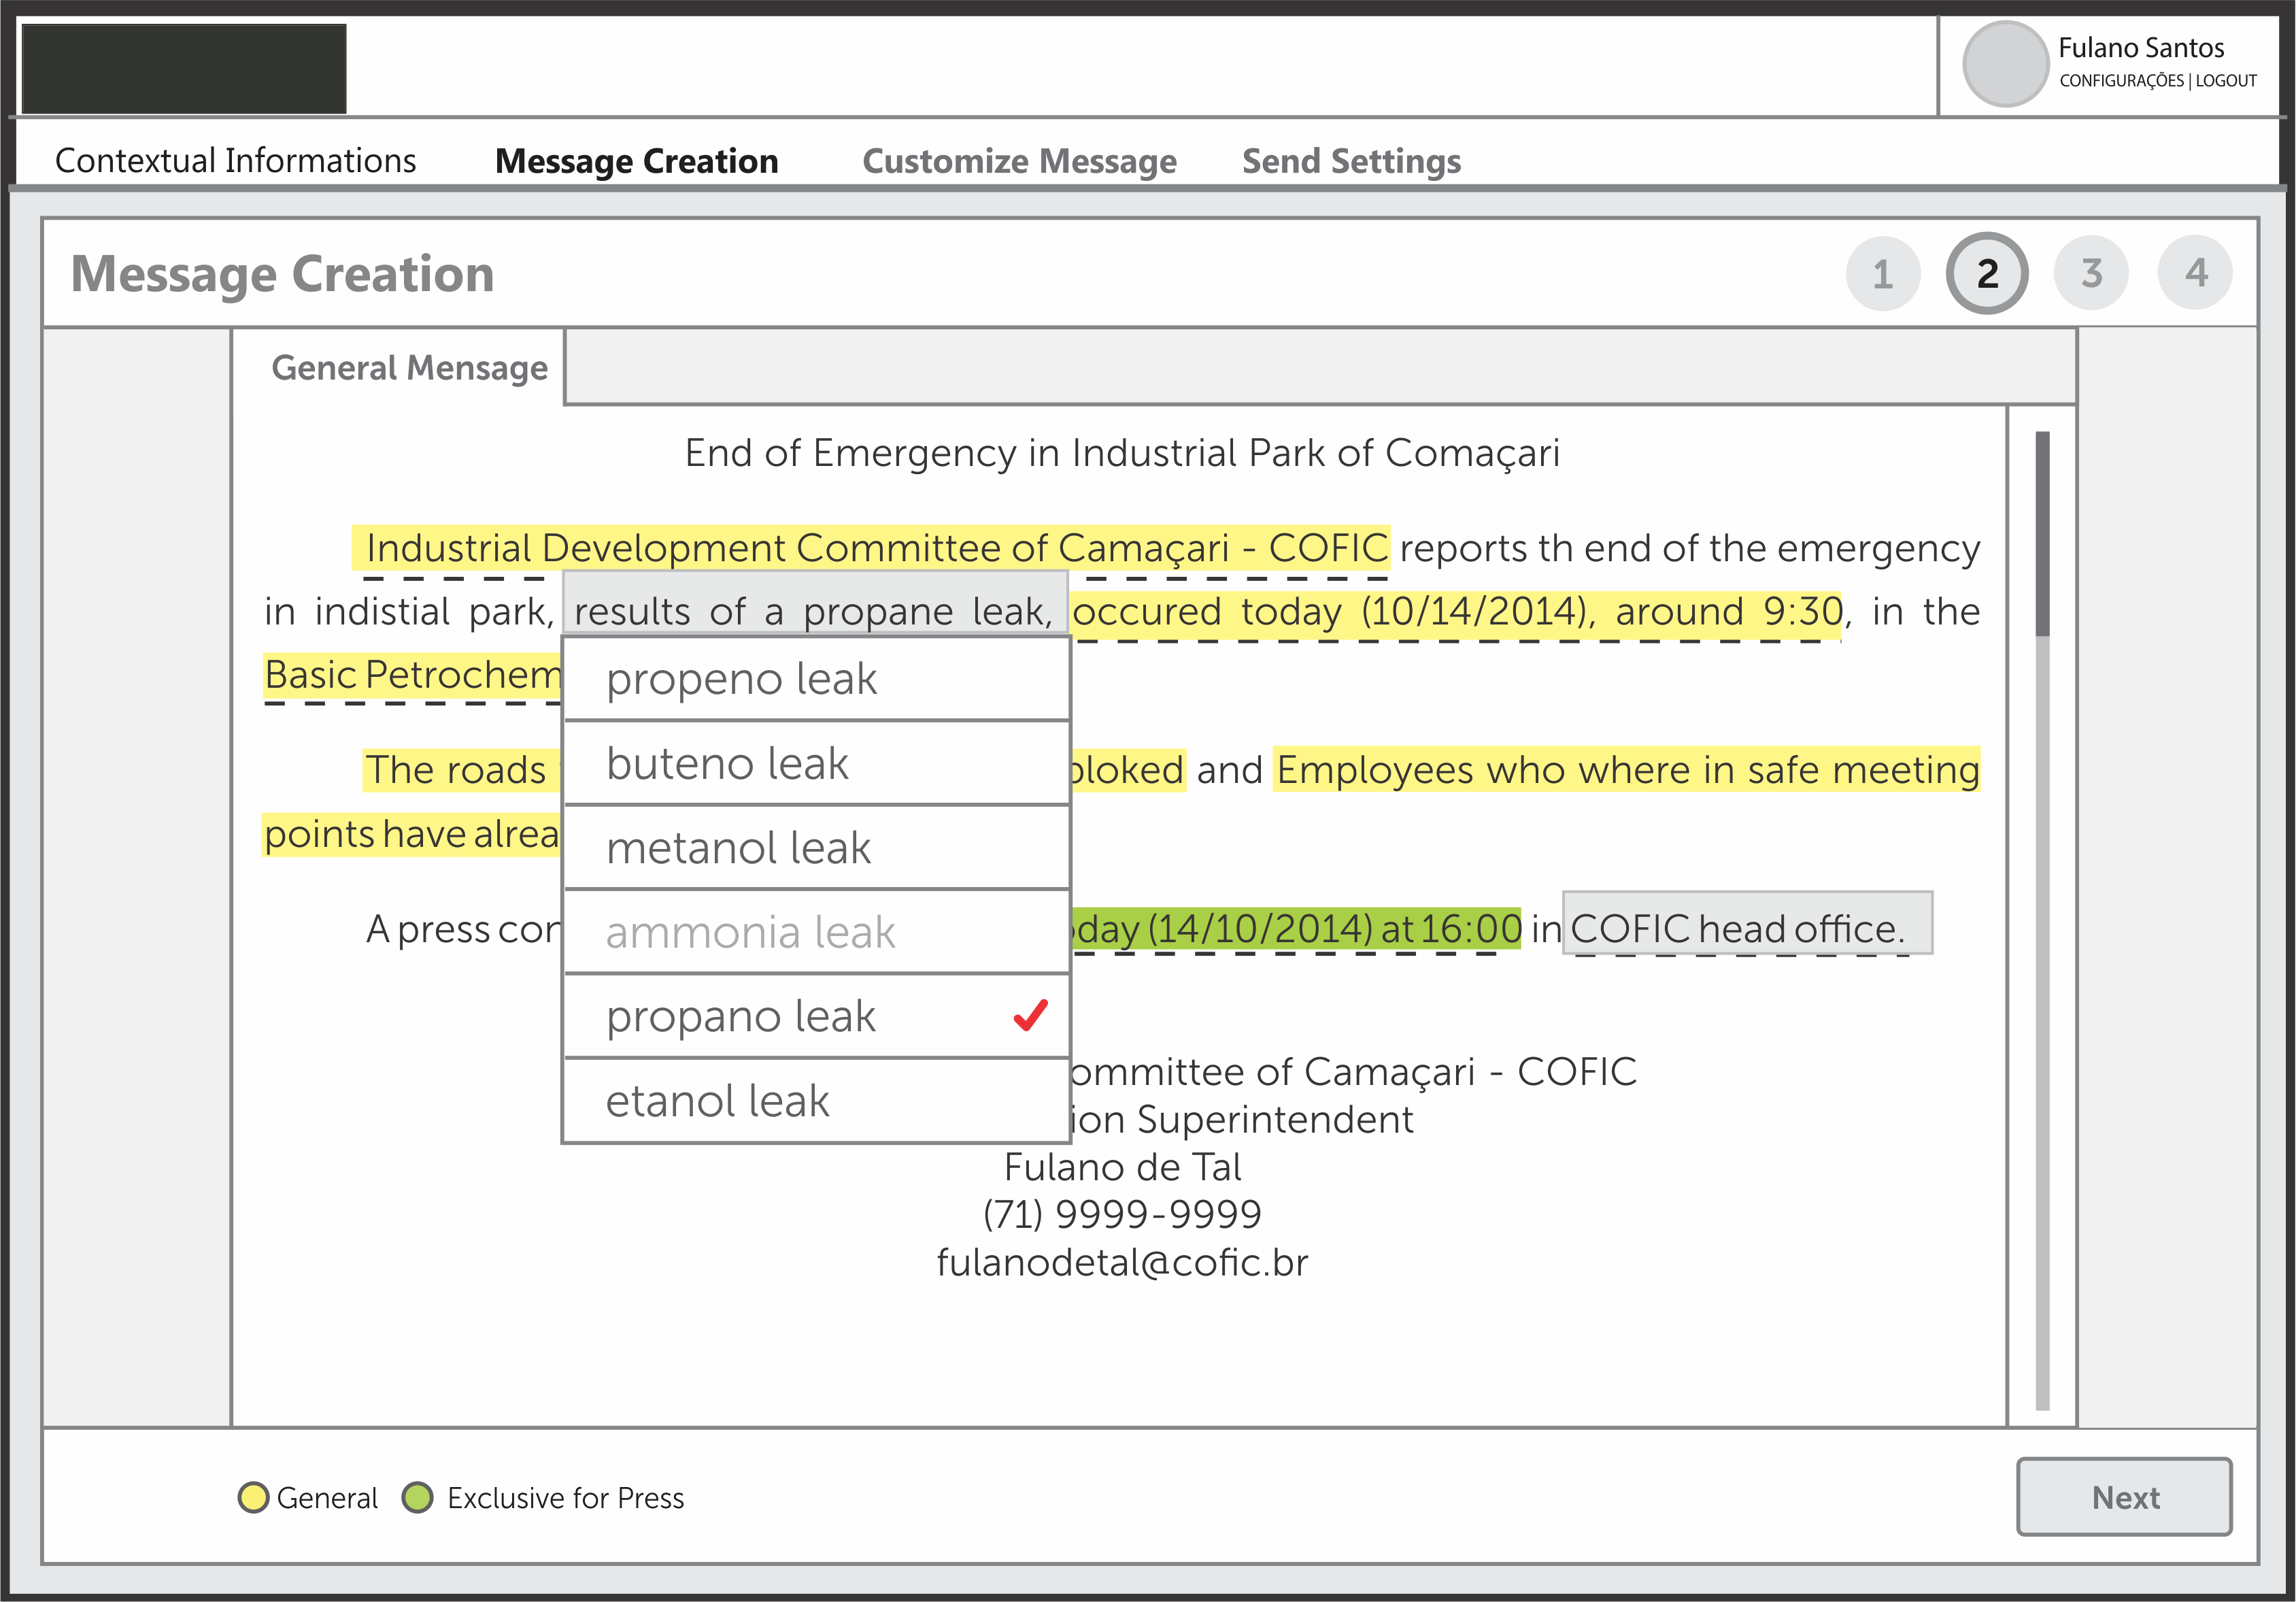
\includegraphics[width=\linewidth]{images/step2.png}
% \caption{User interface to assisted message edition of public communications}
% \label{fig:step2}
% \end{figure}

The next step starts with the system seeking the public communication template that best fits
the current emergency phase. The system generates a editable template (Figure \ref{fig:step2}) based on pre-defined templates (configured according to the information of the first step), taking into consideration the principles of a user interface design pattern called Natural Language Form (NLF) \citep{nlf}. The choice of using NLF was motivated by its high acceptance by our experts partners, who claim that NLF is is very similar to the traditional mode of writing a public communication, which increase the learnability and make the visualisation of the final communication easier.

% \begin{figure}
% \centering
% 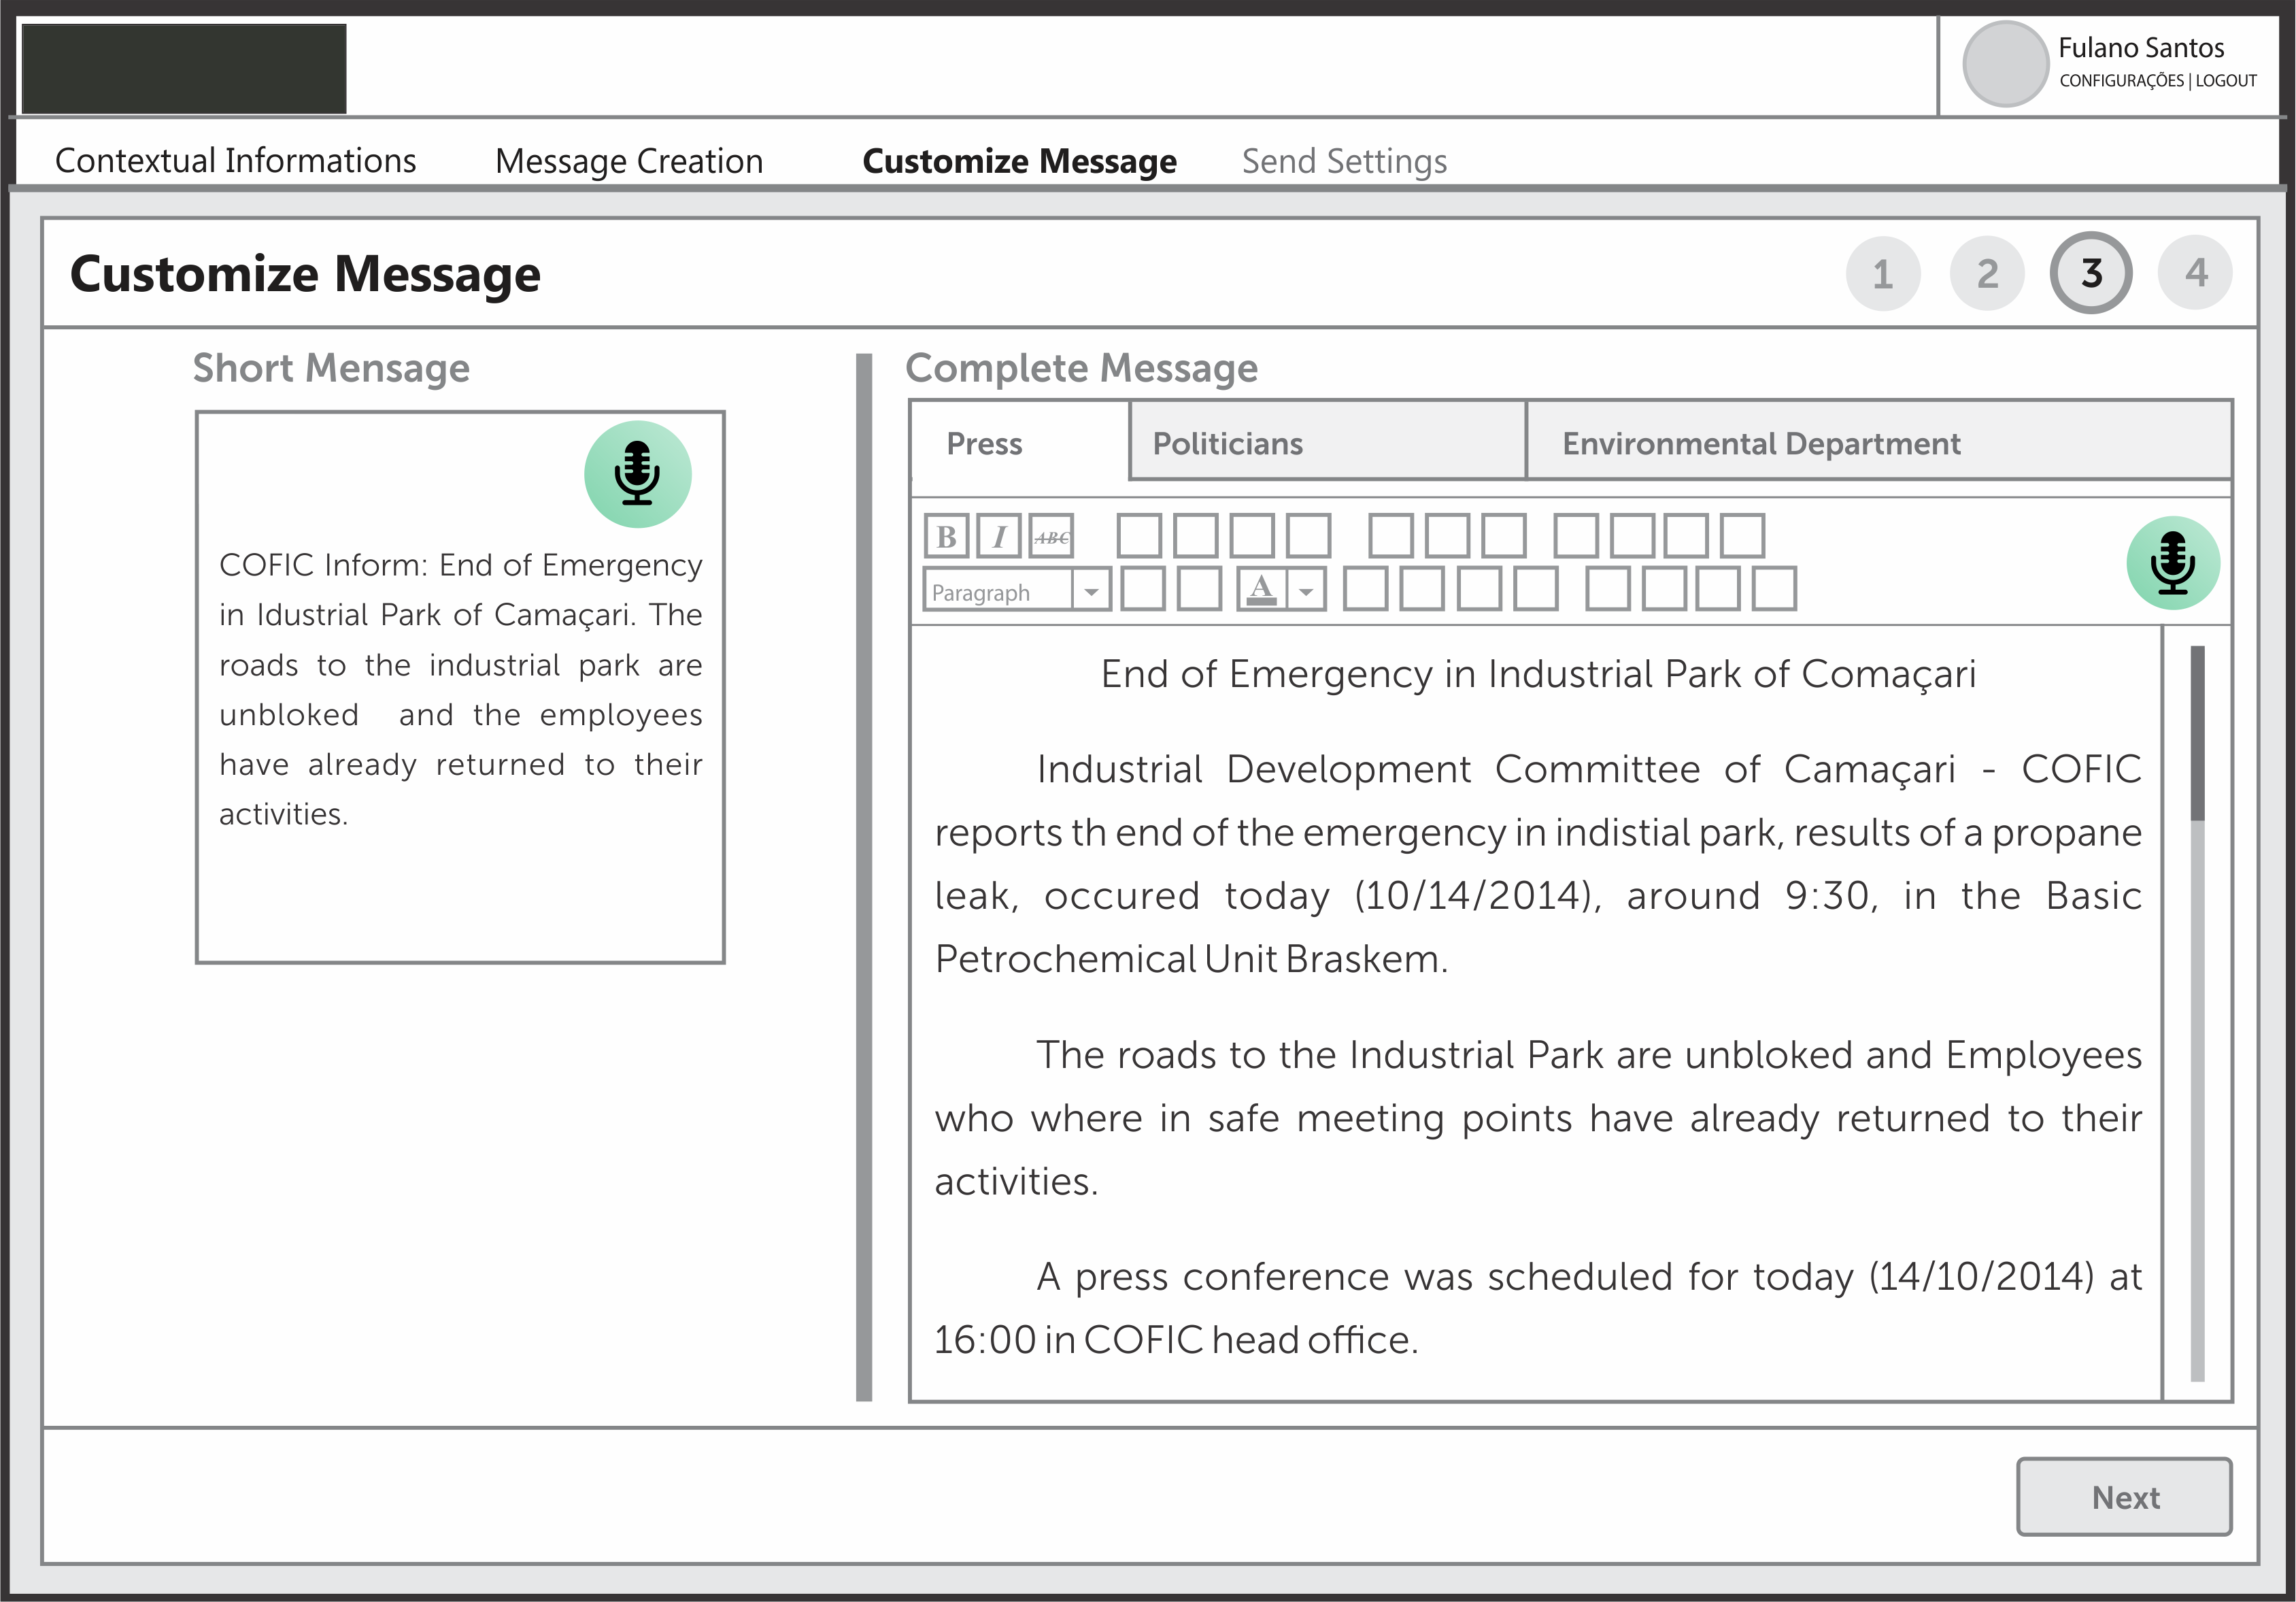
\includegraphics[width=\linewidth]{images/step3.png}
% \caption{User interface to manual customisation of each public communication message}
% \label{fig:step3}
% \end{figure}

In step 3 (Figure \ref{fig:step3}), we propose one screen for customisation of the public communication generated by the template of the step 2. The RESCUER News user can freely edit the text of the public communication and also record audio messages. The possibility of having an audio message was requested by our patterns to allow public communication in radio stations (to be sent attached to e-mail messages) and via RESCUER mobile application for people who have difficulty in reading.

% \begin{figure}
% \centering
% 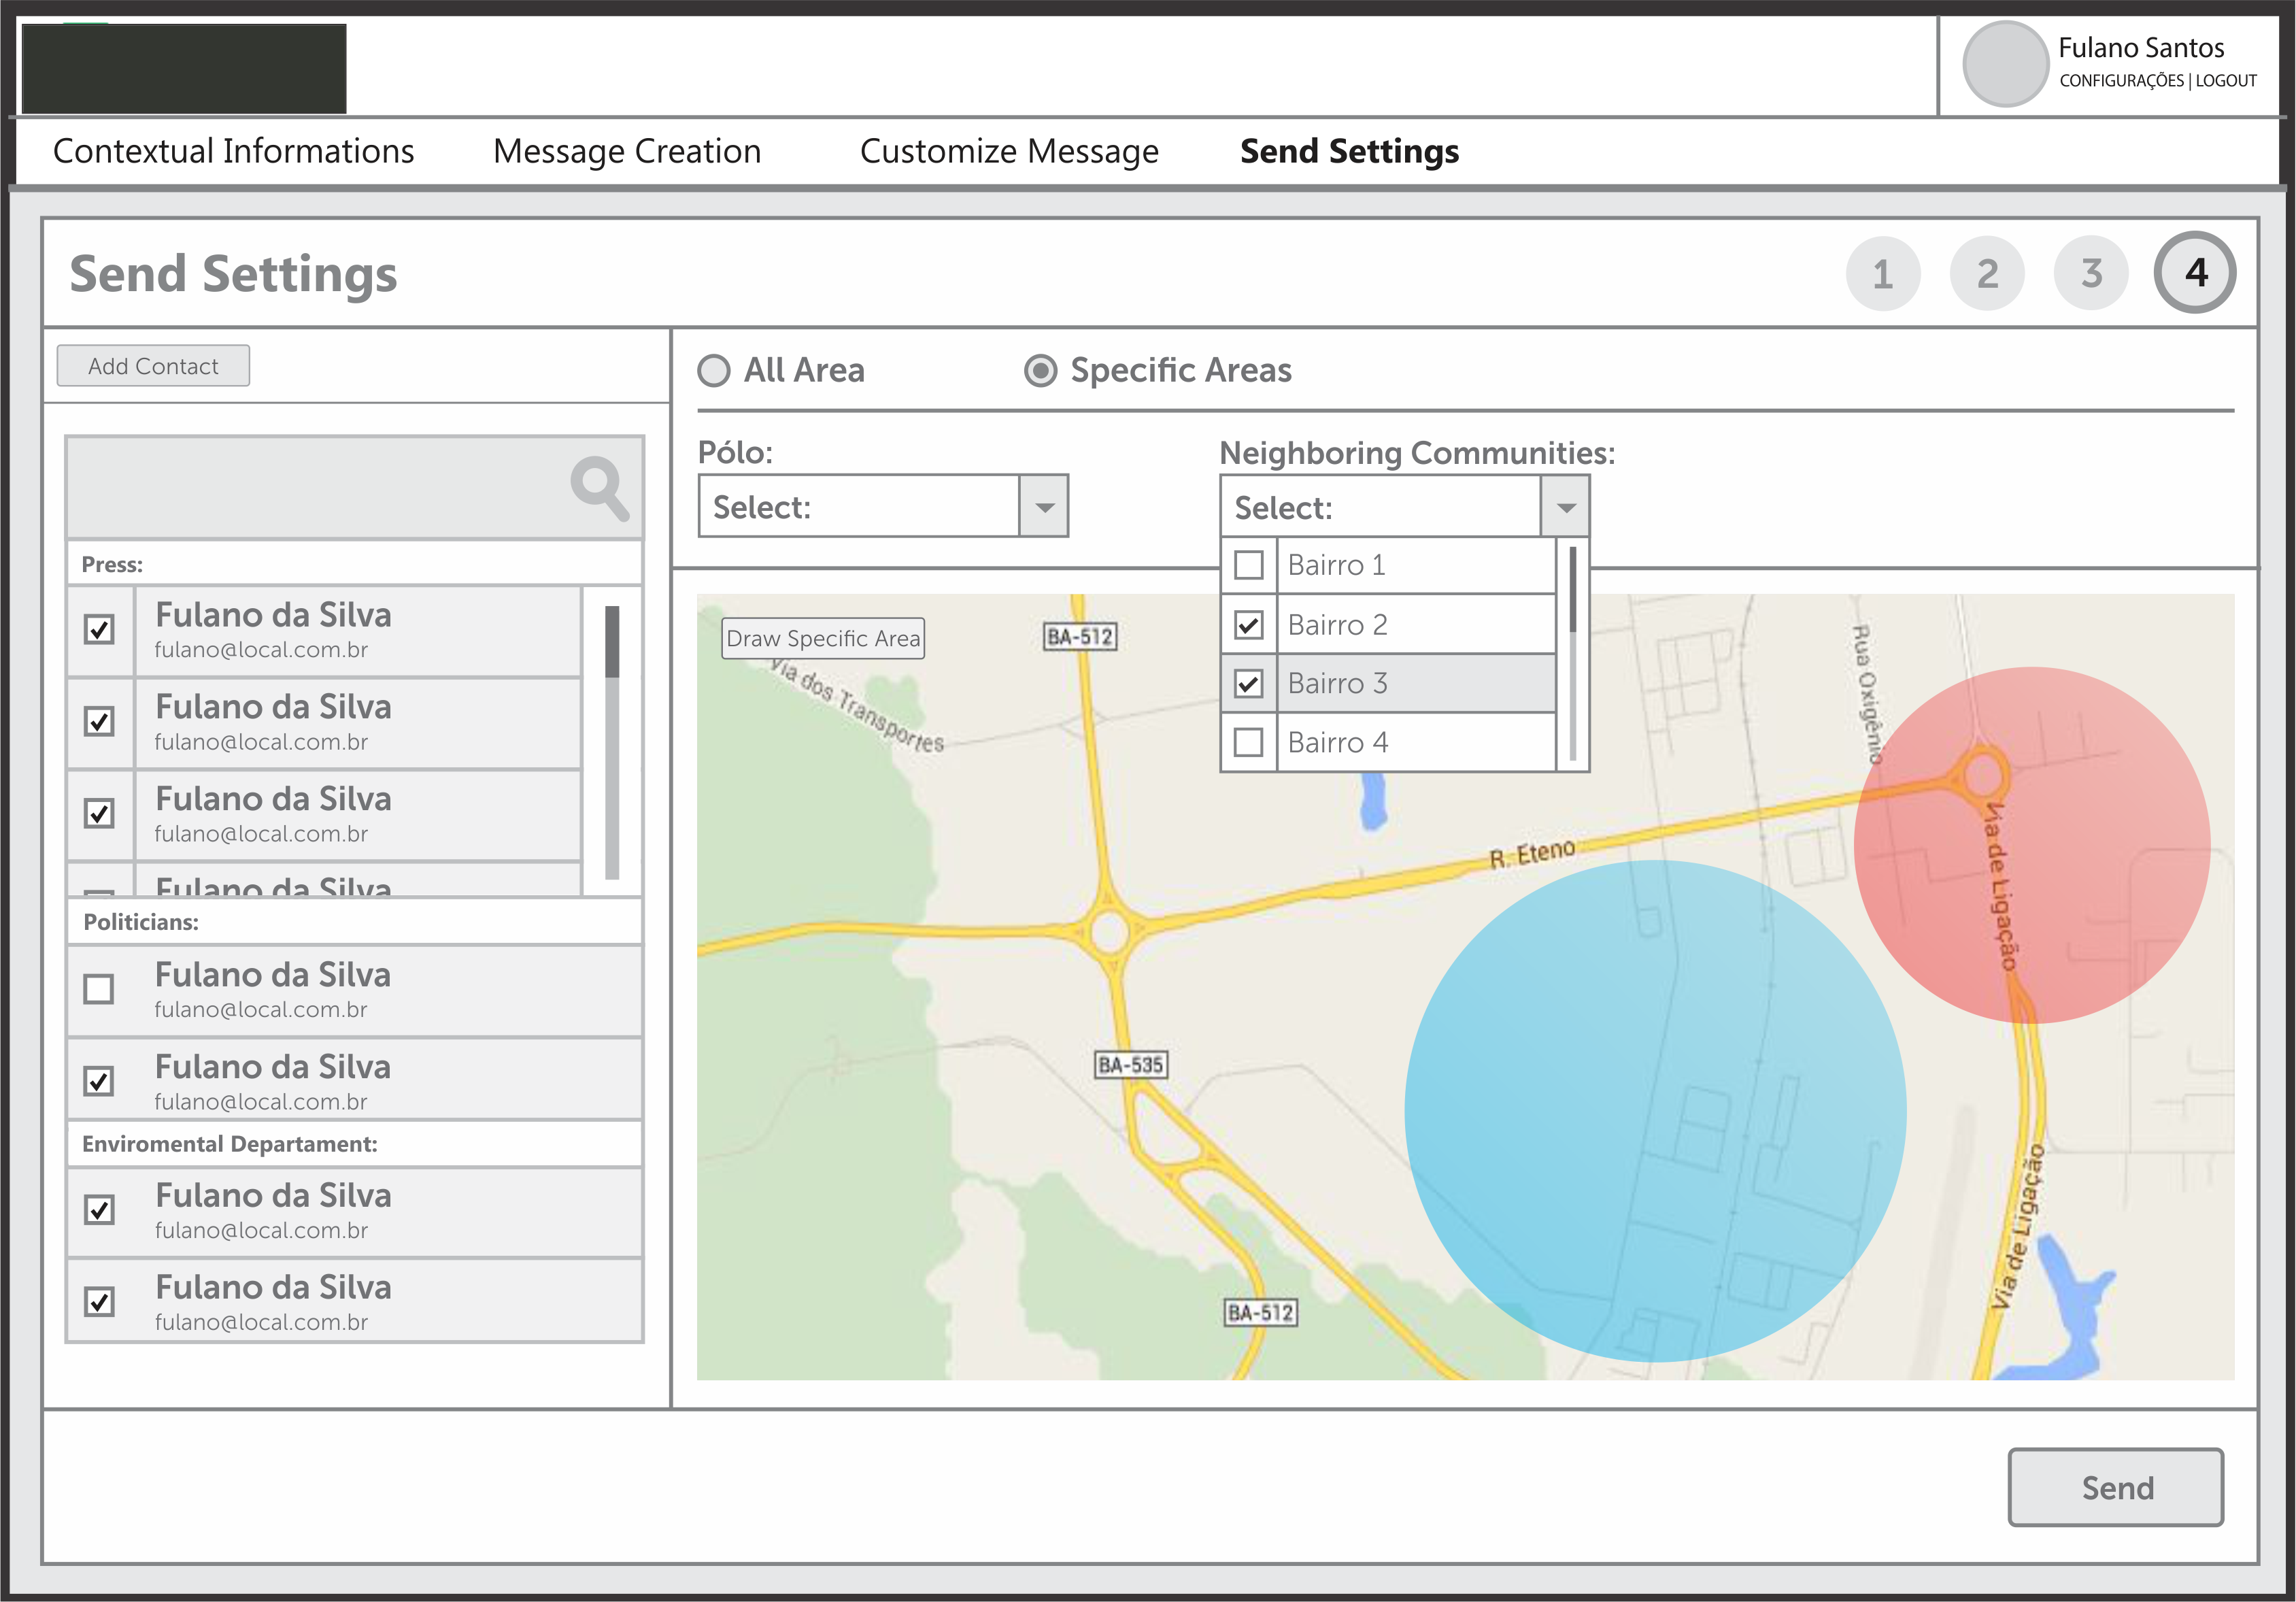
\includegraphics[width=\linewidth]{images/step4.png}
% \caption{Our proposed user interface of target audience sending settings}
% \label{fig:step4}
% \end{figure}

The last step for sending the public communication is to set the sending options. How the message is sent depends on the target audience. For instance, some stakeholders might use RESCUER mobile application (e.g. employees, visitors or neighbour communities) and others might not use it (e.g. politicians, environmental departments and press). Depending on the target audience and communication channels selected in step 1, RESCUER News requests more detailed information in order to send public communications. Figure \ref{fig:step4} shows on the left side how the emergency communicator can use a mailing list previously registered and grouped by type of stakeholder (e.g.,
press, politicians and environmental department) to select the concrete target audience of a specific public communication. On the right side, it is possible to specify areas for sending public communications, by selecting previously registered area or drawing the area in the map, or send them to all users of the RESCUER mobile application regardless of their location.